\documentclass{beamer}

% Theme
\usetheme{Madrid}
\usecolortheme{default}

% Packages
\usepackage{amsmath,amssymb,amsfonts}
\usepackage{graphicx}
\usepackage{xcolor}
\usepackage{tikz}
\usepackage{tkz-euclide}
\usepackage{array}
\usepackage{multirow}
\usepackage{longtable}
\usepackage{lscape}
\usepackage{listings}
\lstset{
    basicstyle=\ttfamily\small,
    keywordstyle=\color{blue},
    commentstyle=\color{gray},
    stringstyle=\color{red},
    showstringspaces=false,
    breaklines=true
}

% Custom macros
\newcommand{\myvec}[1]{\begin{pmatrix}#1\end{pmatrix}}
\newcommand{\brak}[1]{\left( #1 \right)}
\newcommand{\augvec}[3]{%
  \left(\!\begin{array}{@{}*{#1}{r}|*{#2}{r}@{}}#3\end{array}\!\right)
}

% Redefine \vec to bold letters only (no arrow)
\renewcommand{\vec}[1]{\mathbf{#1}}

\title{8.4.22}
\author{EE25BTECH11019 -- Darji Vivek M.}
\date{}

\begin{document}

\begin{frame}
\begin{titlepage}

\end{titlepage}
\end{frame}
\begin{frame}{Question}
\textbf{Question:}\\[2pt]
The radius of the circle passing through the foci of the ellipse
\[
\frac{x^2}{16}+\frac{y^2}{9}=1
\]
and having its centre at $(0,3)$ is -\\[6pt]
\begin{enumerate}
    \item $4$
    \item $3$
    \item $\sqrt{\frac{1}{2}}$
    \item $\frac{7}{2}$
\end{enumerate}
\end{frame}

\begin{frame}{Solution}
Use the matrix form (matrix method). Let $\vec{x}=\myvec{x\\[2pt]y}$. The ellipse is
\[
\vec{x}^\top \vec{V}\,\vec{x}=1,\qquad
\vec{V}=\myvec{\frac{1}{16} & 0\\[2pt]0 & \frac{1}{9}}.
\]
Eigenvalues of $\vec{V}$ (diagonal entries) are
\[
\lambda_1=\frac{1}{16},\qquad \lambda_2=\frac{1}{9}.
\]
For the principal-form ellipse $\vec{x}^\top\vec{V}\vec{x}=1$ the semi-axes satisfy
\[
a^2=\frac{1}{\lambda_1}=16,\qquad b^2=\frac{1}{\lambda_2}=9.
\]
Using the formula for eccentricity.
\[
e=\sqrt{1-\frac{\lambda_1}{\lambda_2}}
=\sqrt{1-\frac{1/16}{1/9}}
=\sqrt{1-\frac{9}{16}}
=\sqrt{\frac{7}{16}}
=\frac{\sqrt7}{4}.
\]
\end{frame}
\begin{frame}{Solution}
The focal distance (from the centre) is \(c = a e\), therefore
\[
c = 4\cdot\frac{\sqrt7}{4}=\sqrt7.
\]
Since \(\vec V\) is diagonal with \(\lambda_1\) along the x-direction, the principal axis unit vector is.

\[
\vec n=\myvec{1\\[2pt]0}.
\]
Thus the foci (in vector form) are
\[
\vec F_1 = c\vec n = \myvec{\sqrt7\\[2pt]0},\qquad
\vec F_2 = -c\vec n = \myvec{-\sqrt7\\[2pt]0}.
\]
\end{frame}
\begin{frame}{Solution}
The required circle has centre $\vec{C}=\myvec{0\\[2pt]3}$ and passes through, say, $\vec{F_1}$. Therefore its radius is
\[
R=\left\|{\vec{F_1}-\vec{C}}\right\|
=\sqrt{\bigl(\sqrt{7}-0\bigr)^2+\bigl(0-3\bigr)^2}
=\sqrt{7+9}
=\sqrt{16}
=\boxed{4}.
\]
\end{frame}
\begin{frame}[fragile]{C code}
\begin{lstlisting}
#include <stdio.h>
#include <math.h>

float circle_radius() {
    // Ellipse: x^2/16 + y^2/9 = 1
    float a2 = 16.0;   // a^2
    float b2 = 9.0;    // b^2
    // Focal distance from origin: c = sqrt(a^2 - b^2)
    float c = sqrt(a2 - b2); // sqrt(7)
    // Foci: (±sqrt(7), 0)
    // Centre of circle: (0, 3)
    // Radius = distance between (sqrt(7), 0) and (0, 3)
    float radius = sqrt((c - 0)*(c - 0) + (0 - 3)*(0 - 3));
    return radius; // should be 4
}

\end{lstlisting}
\end{frame}

\begin{frame}[fragile]{Python}
\begin{lstlisting}[language=Python]
import ctypes
import numpy as np
import matplotlib.pyplot as plt

# Load C shared library
lib = ctypes.CDLL("./15.so")
# Set return type for circle_radius()
lib.circle_radius.restype = ctypes.c_float
# Call the C function
r = lib.circle_radius()
print("Radius of the circle =", r)
# -------------- Plotting --------------
# Ellipse: x^2/16 + y^2/9 = 1
a = 4
b = 3
x = np.linspace(-a, a, 400)
y_top = b * np.sqrt(1 - (x**2 / a**2))
y_bottom = -y_top
\end{lstlisting}
\end{frame}
\begin{frame}[fragile]{Python}
\begin{lstlisting}[language=Python]
# Foci
c = np.sqrt(a**2 - b**2)
F1 = (c, 0)
F2 = (-c, 0)

# Circle centered at (0, 3) passing through (sqrt(7), 0)
theta = np.linspace(0, 2*np.pi, 200)
x_circ = r * np.cos(theta)
y_circ = 3 + r * np.sin(theta)

# Plot ellipse
plt.plot(x, y_top, 'b', label="Ellipse")
plt.plot(x, y_bottom, 'b')

# Plot circle
plt.plot(x_circ, y_circ, 'r', label="Circle")
\end{lstlisting}
\end{frame}
\begin{frame}[fragile]{Python}
\begin{lstlisting}[language=Python]
# Plot foci and center
plt.scatter([F1[0], F2[0]], [F1[1], F2[1]], color='green', label="Foci")
plt.scatter(0, 3, color='black', label="Circle center (0,3)")

# Equal aspect ratio
plt.gca().set_aspect('equal', adjustable='box')
plt.xlabel("x")
plt.ylabel("y")
plt.title("Ellipse and Circle passing through Foci")
plt.grid(True)
plt.legend()
plt.show()
\end{lstlisting}
\end{frame}

\begin{frame}{Pyhton plot}
\begin{figure}[h!]
    \centering
    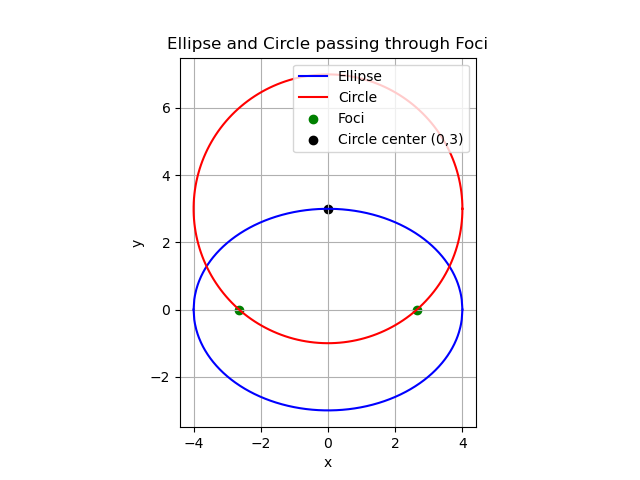
\includegraphics[width=0.75\textwidth]{figs/15.png}
    \caption{plot if p=2,q=2}
    \label{fig:example_image}
\end{figure}
\end{frame}

\end{document}